%%%%%%%%%%%%%%%%%%%%%%%%%%%%%%%%%%%%%%%%%%%%%%%%%%%%%%%%%%%%%%%%%%%%
%% I, the copyright holder of this work, release this work into the
%% public domain. This applies worldwide. In some countries this may
%% not be legally possible; if so: I grant anyone the right to use
%% this work for any purpose, without any conditions, unless such
%% conditions are required by law.
%%%%%%%%%%%%%%%%%%%%%%%%%%%%%%%%%%%%%%%%%%%%%%%%%%%%%%%%%%%%%%%%%%%%

\documentclass{beamer}
\usetheme[faculty=ped,logo=fibeamer/logo/mu/Logo-UC-3.png]{fibeamer} % no extension

\usepackage{algorithm}
\usepackage{algpseudocode}

\usetheme[faculty=ped]{fibeamer}
\usepackage[utf8]{inputenc}
\usepackage[
  main=english, %% By using `czech` or `slovak` as the main locale
                %% instead of `english`, you can typeset the
                %% presentation in either Czech or Slovak,
                %% respectively.
  czech, slovak %% The additional keys allow foreign texts to be
]{babel}        %% typeset as follows:
%%
%%   \begin{otherlanguage}{czech}   ... \end{otherlanguage}
%%   \begin{otherlanguage}{slovak}  ... \end{otherlanguage}
%%
%% These macros specify information about the presentation
\title{Introducción a la Programación} %% that will be typeset on the
\subtitle{Semestre II-2026} %% title page.
\author{Andreina Cota Vidaurre}
%% These additional packages are used within the document:
\usepackage{ragged2e}  % `\justifying` text
\usepackage{booktabs}  % Tables
\usepackage{tabularx}
\usepackage{tikz}      % Diagrams
\usetikzlibrary{calc, shapes, backgrounds}
\usetikzlibrary{positioning, arrows.meta, shadows.blur, shapes.geometric}
\usepackage{amsmath, amssymb}
\usepackage{url}       % `\url`s
\usepackage{listings}  % Code listings
\usepackage{graphicx}
\usepackage{amsmath}
\usepackage[T1]{fontenc}
\usepackage{xcolor}
\usepackage{minted}
\usepackage{pifont}
% \usepackage{adjustbox}


% Definicion de pseudocodigo en espaniol
\lstdefinelanguage{PseudocodigoES}{
    morekeywords={INICIO,FIN,PARA,HACER,SI,ENTONCES,FIN_SI,FIN_PARA,IMPRIMIR},
    sensitive=true,
    morecomment=[l]{//},
    morestring=[b]"
}

% Definicion de pseudocodigo en ingles
\lstdefinelanguage{PseudocodeEN}{
    morekeywords={BEGIN,END,FOR,DO,IF,THEN,END_IF,END_FOR,PRINT},
    sensitive=true,
    morecomment=[l]{//},
    morestring=[b]"
}

\lstset{
    basicstyle=\ttfamily\small,
    keywordstyle=\bfseries,
    columns=fullflexible,
    keepspaces=true,
    showstringspaces=false,
    frame=single,
    xleftmargin=0em,
    framexleftmargin=0em,
    framesep=2pt,
    gobble=4,
    resetmargins=true,
    aboveskip=0pt,
    belowskip=0pt
}

\lstdefinestyle{pythonstyle}{
    language=Python,
    basicstyle=\ttfamily\small,
    keywordstyle=\bfseries,
    commentstyle=\itshape,
    stringstyle=\ttfamily,
    showstringspaces=false,
    columns=fullflexible,
    keepspaces=true,
    frame=single,
    breaklines=true,
    xleftmargin=0em,
    framexleftmargin=0em,
    framesep=2pt,
    aboveskip=0pt,
    belowskip=0pt,
    gobble=4,
    resetmargins=true,
    emph={print,input,int,float,str,bool,len,range},
    emphstyle=\bfseries
}

\lstset{style=pythonstyle}

% Estilos del diagrama
\tikzstyle{iniciofin} = [
    ellipse,
    minimum width=2.5cm,
    minimum height=1cm,
    text centered,
    draw=black,
    fill=blue!25
]

\tikzstyle{proceso} = [
    rectangle,
    rounded corners,
    minimum width=3cm,
    minimum height=1cm,
    text centered,
    draw=black,
    fill=cyan!20
]

\tikzstyle{decision} = [
    diamond,
    aspect=2,
    text centered,
    draw=black,
    fill=yellow!35
]

\tikzstyle{flecha} = [
    thick,
    ->,
    >=Stealth
]

% \definecolor{green_python}{HTML}{52A736}

% \newcolumntype{Y}{>{\raggedright\arraybackslash}X}

\frenchspacing
\begin{document}
  \shorthandoff{-}
  \frame[c]{\maketitle}

% \begin{darkframes}

    \begin{frame}{Estructuras anidadas}
        \begin{itemize}
            \item Introducción
            \item Tipos de estructuras anidadas
            \item Acceso a estructuras anidadas
            \item Recorrido de estructuras anidadas
            \item Ejercicios
            \item Resumen
        \end{itemize}
    \end{frame}

    \begin{frame}{Introducción}
        \begin{itemize}
            \item En el mundo real, la información rara vez está organizada como una lista simple de elementos.
            \item Frecuentemente, la información tiene una estructura jerárquica, es decir, hay datos que contienen otros datos.
            \item Estas estructuras aparecen de forma natural cuando un elemento está compuesto por varios subelementos relacionados entre sí.
            \item Un estudiante puede tener varios ramos y cada ramo varias notas. El universo contiene galaxias; las galaxias contienen sistemas estelares; y estos contienen estrellas y sus planetas.
        \end{itemize}
    \end{frame}

    \begin{frame}{Introducción}
        \begin{figure}
            \centering
            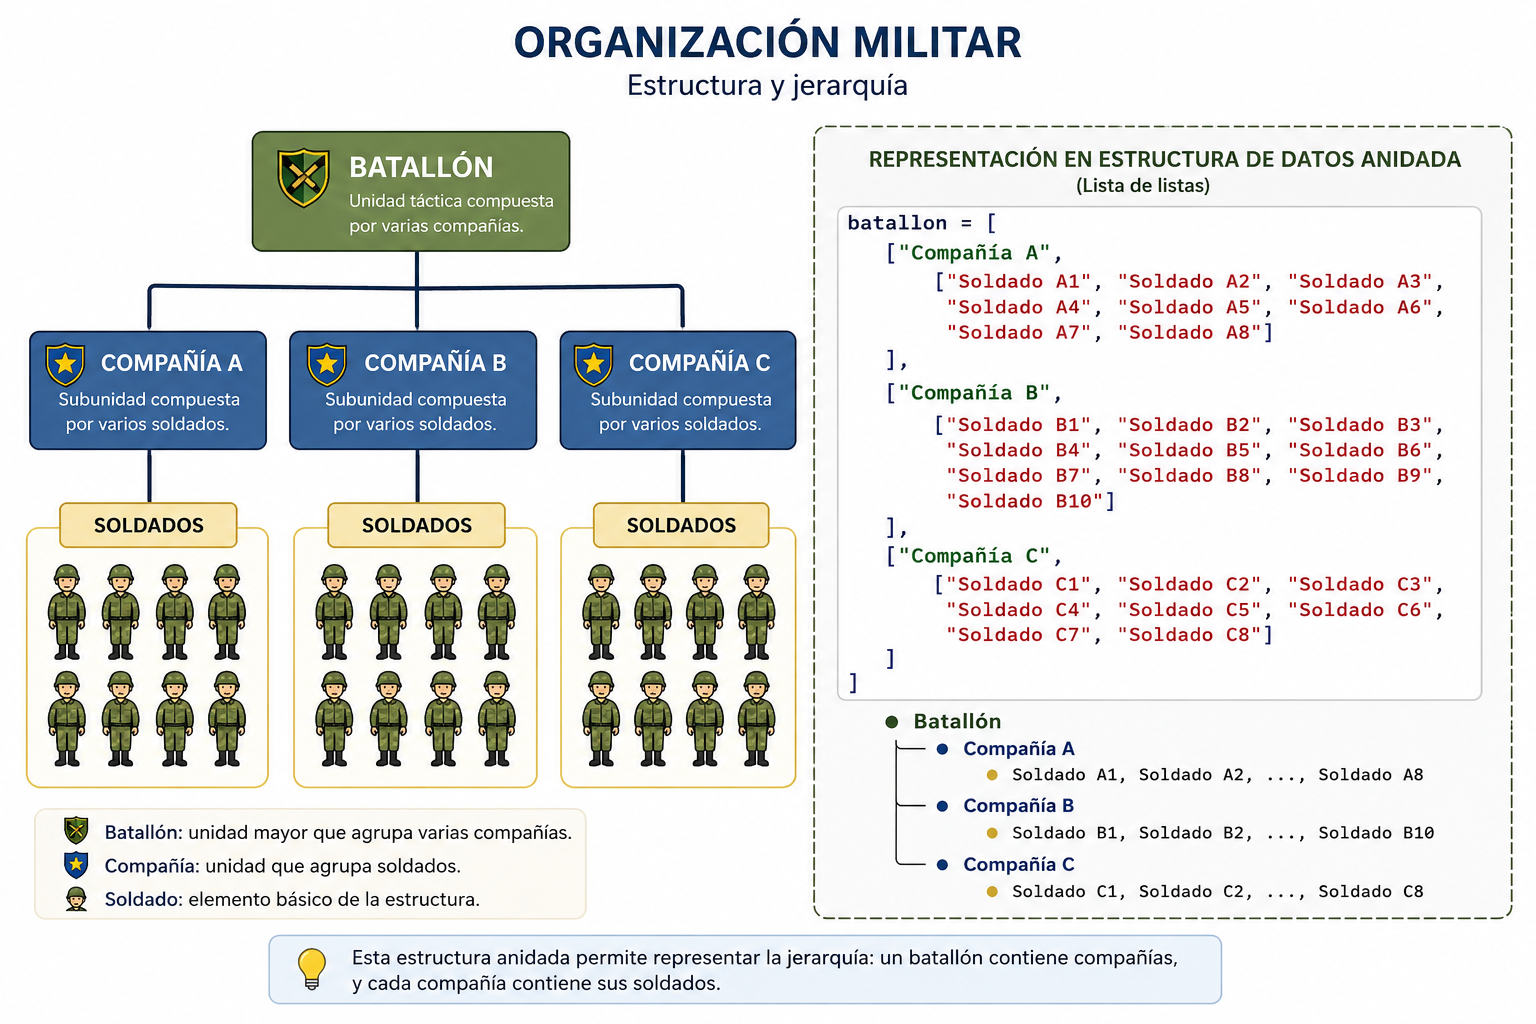
\includegraphics[width=\linewidth]{resources/organizacion_militar.png}
        \end{figure}
    \end{frame}

    \begin{frame}{Introducción}
        \begin{itemize}
            \item Para representar esa \textbf{estructura jerárquica}, es necesario utilizar estructuras anidadas.
            \item Una estructura anidada es una colección que contiene otras colecciones.
            \item En Python, una estructura puede contener distintos tipos de datos y otras estructuras.
            \item Algunos ejemplos de estructuras anidadas son: 
            \begin{itemize}
                \item Listas de listas
                \item Listas de tuplas
                \item Tuplas de listas
                \item Tuplas de tuplas
                \item Diccionarios de listas
                \item Diccionarios de diccionarios
            \end{itemize}
            % \item Estas estructuras permiten representar relaciones del tipo: datos dentro de datos.
        \end{itemize}
    \end{frame}

    \begin{frame}[fragile,t]{Tipos de estructuras anidadas}
        \begin{itemize}
            \item \textbf{Lista de listas}: Lista donde cada elemento también es una lista.
            \begin{minted}[xleftmargin=-2cm, frame=leftline,fontsize=\small]{python}
            # Notas de 3 alumnos en 4 pruebas
            notas = [[85, 90, 78, 92],
                     [70, 65, 88, 75],
                     [95, 100, 91, 88]]
            \end{minted}
            \item \textbf{Lista de tuplas}: Lista donde cada elemento es una tupla.
            \begin{minted}[xleftmargin=-2cm, frame=leftline,fontsize=\small]{python}
            # Posiciones de objetivos (latitud, longitud)
            objetivos = [(-33.45, -70.67),
                         (-33.46, -70.65),
                         (-33.44, -70.70)]
            \end{minted}
        \end{itemize}
    \end{frame}

    \begin{frame}[fragile,t]{Tipos de estructuras anidadas}
        \begin{itemize}
            \item \textbf{Tupla de tuplas}: Tupla donde cada elemento es una tupla.
            \begin{minted}[xleftmargin=-2cm, frame=leftline,fontsize=\small]{python}
            # Tabla periódica (símbolo, número atómico, masa)
            elementos = (("H", 1, 1.008),
                         ("He", 2, 4.003),
                         ("Li", 3, 6.941))
            \end{minted}
            \item \textbf{Tupla de listas}: Tupla donde cada elemento es una lista.
            \begin{minted}[xleftmargin=-2cm, frame=leftline,fontsize=\small]{python}
            # 3 turnos fijos, cada uno con lista de tareas variable
            turnos = (["patrulla norte", "relevo 06:00"],
                      ["guardia sur"],
                      ["logística", "comunicaciones"])
            \end{minted}
        \end{itemize}
    \end{frame}

    \begin{frame}[fragile, t]{Cómo acceder a los elementos}
        \begin{minted}[xleftmargin=-2cm, frame=leftline,fontsize=\small]{python}
            matriz = [
              [10, 20, 30],    # fila 0
              [40, 50, 60],    # fila 1
              [70, 80, 90]     # fila 2
            ]
            \end{minted}
        \begin{itemize}
            \item Una estructura anidada es una colección cuyo contenido son otras colecciones.
            \item Se puede visualizar como una tabla: tiene filas y columnas.
            \item Para llegar a un valor específico, necesitas dos pasos:
            \begin{enumerate}
                \item Elegir la fila
                \item Elegir el elemento de esa fila
            \end{enumerate}
        \end{itemize}
    \end{frame}

    \begin{frame}[fragile, t]{El primer corchete: elige la fila}
        \begin{itemize}
            \item \mintinline{python}{matriz[i]} selecciona la fila completa en la posición \mintinline{python}{i}.
            \item No devuelve un número; devuelve la lista completa.
            \item Es el primer nivel de acceso
        \end{itemize}
        \begin{minted}[xleftmargin=-2cm, frame=leftline,fontsize=\small]{python}
                matriz = [[10, 20, 30],
                          [40, 50, 60],
                          [70, 80, 90]]
                
                # ¿Cómo se lee?  matriz[i]
                #   i → elige la lista interna (la fila)
                
                print(matriz[0])       # [10, 20, 30]  ← toda la fila 0
        \end{minted}
    \end{frame}

    \begin{frame}[fragile, t]{El segundo corchete: elige el elemento}
        \begin{itemize}
            \item \mintinline{python}{matriz[i][j]} accede a la fila \mintinline{python}{i} y selecciona el elemento en la posición \mintinline{python}{j}.
            \item De esa forma, obtienes un valor de la matriz, de la posición \mintinline{python}{(i, j)}
        \end{itemize}
        \begin{minted}[xleftmargin=-2cm, frame=leftline,fontsize=\small]{python}
            # estructura[fila][columna]  →  estructura[i][j]
            matriz = [[10, 20, 30],
                      [40, 50, 60],
                      [70, 80, 90]]
            # ¿Cómo se lee?  matriz[i][j]
            #   i → elige la lista interna (la fila)
            #   j → elige el elemento dentro de esa lista
            print(matriz[1])      # [40, 50, 60]  ← toda la fila 1
            print(matriz[1][2])   # 60 ← fila 1, columna 2
            print(matriz[-1][0])  # 70 ← última fila, primer elemento
            \end{minted}
    \end{frame}

    \begin{frame}[fragile, t]{Cómo acceder a los elementos}
        \begin{minted}[xleftmargin=-2cm, frame=leftline,fontsize=\small]{python}
            puntos = [(1, 2), (3, 4), (5, 6)]
            
            print(puntos[0])      # (1, 2)   ← la primera tupla completa
            print(puntos[1][0])  # 3        ← segundo punto, coordenada x
            print(puntos[2][1])  # 6        ← tercer punto, coordenada y
            \end{minted}
    \end{frame}

    \begin{frame}[fragile, t]{Acceder a estructuras anidadas: Regla general}
        \begin{itemize}
            \item El primer corchete siempre indica la fila.
            \item El segundo corchete siempre indica la posición dentro de la fila.
            \item La sintaxis es: \mintinline{python}{[i][j]}
            \item El nombre de los índices puede ser cualquier nombre: \mintinline{python}{[fila][columna]} 
        \end{itemize}
    \end{frame}

    \begin{frame}[fragile, t]{Ejemplos: multiplicación de matrices}
        \begin{minted}[xleftmargin=-2cm, frame=leftline,fontsize=\small]{python}
            # Sistema de ecuaciones  2x + y = 5 / x + 3y = 10
            # Representado como matriz aumentada
            sistema = [[2, 1, 5],
                       [1, 3, 10]]
            
            # Acceder al coeficiente de y en la segunda ecuación
            coef_y_ec2 = sistema[1][1]   # → 3
        \end{minted}
    \end{frame}

    \begin{frame}[fragile, t]{Ejemplos: Tabla periódica}
        Los datos de los elementos no cambian: símbolo, número atómico, masa
        \begin{minted}[xleftmargin=-2cm, frame=leftline,fontsize=\small]{python}
            # (símbolo, número_atómico, masa_molar, electronegatividad)
            tabla = (("H",  1,   1.008,  2.20),
                     ("C",  6,  12.011,  2.55),
                     ("N",  7,  14.007,  3.04),
                     ("O",  8,  15.999,  3.44),
                     ("Na", 11, 22.990,  0.93))
    
            # Masa molar del nitrógeno
            print(tabla[2][2])  # 14.007
        \end{minted}
    \end{frame}

    \begin{frame}[fragile, t]{Ejemplos: Horario semanal de clases}
        Los días son filas; los bloques son las columnas
        \begin{minted}[xleftmargin=-2cm, frame=leftline,fontsize=\small]{python}
            # Horario[día][bloque]  (0=Lunes...4=Viernes)
            horario = [
                ["Álgebra", "Programación",   "Física"],  # Lunes
                ["Química", "Educación Fís.", "Inglés"],  # Martes
                ["Álgebra", "Programación", "Historia"],  # Miércoles
                ["Física",  "Química",  "Programación"],  # Jueves
                ["Inglés",  "Álgebra",    "Literatura"]   # Viernes
            ]
            # ¿Qué hay el miércoles en el segundo bloque?
            print(horario[2][1])  # "Programación"
        \end{minted}
    \end{frame}

    \begin{frame}[fragile, t]{Ejemplos: Orden de batalla}
        Una unidad mayor contiene unidades menores. Esa jerarquía se representa directamente con una lista de listas.
        \begin{minted}[xleftmargin=-2cm, frame=leftline,fontsize=\small]{python}
            # Brigada → Batallones → Compañías
            # orbat[batallón][compañía]
            orbat = [
            ["Cía. A/I Btn", "Cía. B/I Btn", "Cía. C/I Btn"], # I Batallón
            ["Cía. A/II Btn", "Cía. B/II Btn"],      # II Batallón
            ["Cía. Ingenieros", "Cía. Comunicaciones"] # Apoyo
            ]
            
            # ¿Qué unidad es la segunda compañía del I Batallón?
            print(orbat[0][1])  # "Cía. B/I Btn"
        \end{minted}
    \end{frame}

    \begin{frame}[fragile,t]{Cómo acceder a los elementos}
        \begin{center}
        \begin{tabular}{|p{3cm}|p{3cm}|p{3cm}|}
        \hline
        \textbf{Tipo} & \textbf{Acceso} & \textbf{Ejemplo} \\
        \hline
        \mintinline{python}{lista[lista]}   & \mintinline{python}{m[i][j]} & Matriz de 3 x 3 \\ \hline
        \mintinline{python}{lista[tupla]} & \mintinline{python}{p[i][j]}  & Lista de puntos \\ \hline
        \mintinline{python}{tupla[tupla]} & \mintinline{python}{t[i][j]} & Tabla de constantes \\ \hline
        \end{tabular}
        \end{center}
    \end{frame}

    \begin{frame}[fragile, t]{Cómo recorrer las estructuras anidadas}
        \begin{itemize}
            \item Para recorrer toda la estructura se utilizan dos bucles:
            \begin{enumerate}
                \item El externo avanza por las filas (cambia \mintinline{python}{i})
                \item El interno avanza por los elementos de cada fila (cambia \mintinline{python}{j})
            \end{enumerate}
            \item El orden de visita comienza por la fila
        \end{itemize}
    \end{frame}

    \begin{frame}[fragile, t]{Cómo recorrer las estructuras anidadas}
        Recorrer con \mintinline{python}{for} anidados
        \begin{minted}[xleftmargin=-2cm, frame=leftline,fontsize=\small]{python}
            matriz = [
                [100, 110, 120], 
                [130, 140, 150], 
                [160, 170, 180]
            ]
            for fila in matriz:
                print(f"La fila es: {fila}")
                for valor in fila:
                    print(f"El valor de la fila: {fila} es: {valor}")
        \end{minted}
    \end{frame}

    \begin{frame}[fragile, t]{Cómo recorrer las estructuras anidadas}
        Recorrer con \mintinline{python}{for} anidados y \mintinline{python}{enumerate}
        \begin{minted}[xleftmargin=-2cm, frame=leftline,fontsize=\small]{python}
            matriz = [
                [100, 110, 120], 
                [130, 140, 150], 
                [160, 170, 180]
            ]
            for i, fila in enumerate(matriz):
                for j, valor in enumerate(fila):
                    print(f"La matriz[{i}][{j}] = {valor}")
            \end{minted}
    \end{frame}

    \begin{frame}[fragile, t]{Ejercicios: Promedio de notas por estudiante}
        Tienes una lista de listas en la que cada fila representa a un estudiante y cada columna representa la nota de una prueba.
        \begin{minted}[xleftmargin=-2cm, frame=leftline,fontsize=\small]{python}
            notas = [
                [5.5, 6, 4.5, 6.7], 
                [5, 4.8, 6, 3],
                [5.8, 7, 6.2, 5.9]
            ]
        \end{minted}
        
        Realizar un programa que:
        \begin{enumerate}
            \item Muestre el promedio de cada estudiante.
            \item Muestre qué estudiante obtuvo el mayor promedio
            \item Muestre cuántos estudiantes aprobaron, considerando que el promedio es $\geq$ 4.
        \end{enumerate}
    \end{frame}

    \begin{frame}[fragile, t]{Ejercicios: Promedio de notas por estudiante}
        \begin{enumerate}
            \item Muestre el promedio de cada estudiante.
        \end{enumerate}
        \begin{minted}[xleftmargin=-2cm, frame=leftline,fontsize=\small]{python}
            notas = [
                [5.5, 6, 4.5, 6.7], 
                [5, 4.8, 6, 3],
                [5.8, 7, 6.2, 5.9]
            ]
            for i, nota_est in enumerate(notas, start=1):
                promedio = sum(nota_est) / len(nota_est)
                print(f"El estudiante: {i} tiene promedio: {promedio})
            \end{minted}
    \end{frame}

    \begin{frame}[fragile, t]{Ejercicios: Promedio de notas por estudiante}
        \begin{enumerate}
            \item Muestre el promedio de cada estudiante.
            \item Muestre qué estudiante obtuvo el mayor promedio
        \end{enumerate}
        \begin{minted}[xleftmargin=-2cm, frame=leftline,fontsize=\small]{python}
                notas = [
                    [5.5, 6, 4.5, 6.7], 
                    [5, 4.8, 6, 3],
                    [5.8, 7, 6.2, 5.9]
                ]
                mayor_promedio = 0
                for i, nota_est in enumerate(notas, start=1):
                    promedio = sum(nota_est) / len(nota_est)
                    mayor_promedio = max(mayor_promedio, promedio)
                print(f"El mayor promedio es: {mayor_promedio}")
        \end{minted}
    \end{frame}

    \begin{frame}[fragile, t]{Ejercicios: Promedio de notas por estudiante}
        \begin{enumerate}
            \item Muestre el promedio de cada estudiante.
            \item Muestre qué estudiante obtuvo el mayor promedio
            \item Muestre cuántos estudiantes aprobaron, considerando que el promedio es $\geq$ 4.
        \end{enumerate}
        \begin{minted}[xleftmargin=-2cm, frame=leftline,fontsize=\small]{python}
            notas = [[5.5, 6, 4.5, 6.7], 
                    [5, 4.8, 6, 3],
                    [5.8, 7, 6.2, 5.9]]
            num_aprobados = 0
            for i, nota_est in enumerate(notas, start=1):
                promedio = sum(nota_est) / len(nota_est)
                if promedio >= 4:
                    num_aprobados += 1
            print(f"El número de estudiantes aprobados es: {nun_aprobados}")
            \end{minted}
    \end{frame}

    \begin{frame}[fragile, t]{Ejercicios: Batallon militar}
        Se tiene la siguiente organización
        \begin{minted}[xleftmargin=-2cm, frame=leftline,fontsize=\small]{python}
            batallon = [
                ["Compania A", 35],
                ["Compania B", 42],
                ["Compania C", 28]
            ]
        \end{minted}
        Cada lista representa: \mintinline{python}{[nombre, n_soldados]}. Realizar un programa que:
        \begin{enumerate}
            \item Muestre todas las compañías
            \item Calcule el total de soldados
            \item Determine qué compañía tiene más soldados
        \end{enumerate}
    \end{frame}

    \begin{frame}[fragile, t]{Ejercicios: Batallon militar}
        \begin{enumerate}
            \item Muestre todas las compañías
        \end{enumerate}
        \begin{minted}[xleftmargin=-2cm, frame=leftline,fontsize=\small]{python}
            batallon = [
                ["Compania A", 35],
                ["Compania B", 42],
                ["Compania C", 28]
            ]
            for compania in batallon:
                nombre_compania = ______________
                print(f"El nombre de la compañía es: {nombre_compania}")
            \end{minted}
    \end{frame}

    \begin{frame}[fragile, t]{Ejercicios: Batallon militar}
        \begin{enumerate}
            \item Muestre todas las compañías
        \end{enumerate}
        \begin{minted}[xleftmargin=-2cm, frame=leftline,fontsize=\small]{python}
            batallon = [
                ["Compania A", 35],
                ["Compania B", 42],
                ["Compania C", 28]
            ]
            companias = []
            for compania in batallon:
                nombre_compania = _____________
                companias.append(______)
            print(f"Las compañías son: {companias}")
            \end{minted}
    \end{frame}

    \begin{frame}[fragile, t]{Ejercicios: Batallon militar}
        \begin{enumerate}
            \item Muestre todas las compañías
            \item Calcule el total de soldados
        \end{enumerate}
        \begin{minted}[xleftmargin=-2cm, frame=leftline,fontsize=\small]{python}
            batallon = [
                ["Compania A", 35],
                ["Compania B", 42],
                ["Compania C", 28]
            ]
            total_soldados = 0
            for compania in batallon:
                total_soldados += _________
                
            print(f"El total de soldados es: {_____} ")
        \end{minted}
    \end{frame}

    \begin{frame}[fragile, t]{Ejercicios: Batallon militar}
        \begin{enumerate}
            \item Muestre todas las compañías
            \item Calcule el total de soldados
            \item Determina qué compañía tiene más soldados
        \end{enumerate}
        \begin{minted}[xleftmargin=-2cm, frame=leftline,fontsize=\small]{python}
            batallon = [["Compania A", 35],
                        ["Compania B", 42],
                        ["Compania C", 28]]
            max_soldados = 0
            nombre_compania = ""
            for compania in batallon:
                n_soldados = __________
                if n_soldados > max_soldados:
                    nombre_compania = ________
            print(f"La compañía {nombre_compania} tiene más soldados.")
            \end{minted}
    \end{frame}
    
\end{document}
